\documentclass{book}

\newcommand{\vcsbeam}{{\sc VCSBeam}}

\title{\vcsbeam{} Documentation}
\author{Dr. Sammy McSweeney}

\usepackage{amsmath}
\usepackage{fullpage}
\usepackage{listings}
\usepackage{graphicx}
\usepackage{hyperref}
\usepackage{natbib}
\usepackage{makeidx}
\usepackage{listings}
\usepackage{color}

\definecolor{mygreen}{rgb}{0,0.6,0}
\definecolor{mygray}{rgb}{0.5,0.5,0.5}
\definecolor{mymauve}{rgb}{0.58,0,0.82}

\bibliographystyle{chicago}

\lstset{
  backgroundcolor=\color{white},   % choose the background color; you must add \usepackage{color} or \usepackage{xcolor}; should come as last argument
  basicstyle=\footnotesize\ttfamily, % the size of the fonts that are used for the code
  breakatwhitespace=false,         % sets if automatic breaks should only happen at whitespace
  breaklines=true,                 % sets automatic line breaking
  captionpos=b,                    % sets the caption-position to bottom
  commentstyle=\color{mygreen},    % comment style
  deletekeywords={...},            % if you want to delete keywords from the given language
  escapeinside={\%*}{*)},          % if you want to add LaTeX within your code
  extendedchars=true,              % lets you use non-ASCII characters; for 8-bits encodings only, does not work with UTF-8
  frame=single,	                   % adds a frame around the code
  keepspaces=true,                 % keeps spaces in text, useful for keeping indentation of code (possibly needs columns=flexible)
  keywordstyle=\color{blue},       % keyword style
  language=Octave,                 % the language of the code
  morekeywords={*,...},            % if you want to add more keywords to the set
  numbers=none,                    % where to put the line-numbers; possible values are (none, left, right)
  numbersep=5pt,                   % how far the line-numbers are from the code
  numberstyle=\tiny\color{mygray}, % the style that is used for the line-numbers
  rulecolor=\color{black},         % if not set, the frame-color may be changed on line-breaks within not-black text (e.g. comments (green here))
  showspaces=false,                % show spaces everywhere adding particular underscores; it overrides 'showstringspaces'
  showstringspaces=false,          % underline spaces within strings only
  showtabs=false,                  % show tabs within strings adding particular underscores
  stepnumber=2,                    % the step between two line-numbers. If it's 1, each line will be numbered
  stringstyle=\color{mymauve},     % string literal style
  tabsize=2,	                   % sets default tabsize to 2 spaces
  title=\lstname                   % show the filename of files included with \lstinputlisting; also try caption instead of title
}

\setcounter{secnumdepth}{4}
\setcounter{tocdepth}{4}

\hypersetup{
    colorlinks=true,
    linkcolor=blue,
    filecolor=blue,
    citecolor=blue,
}

\makeindex

\newcommand{\pd}[2]{\ensuremath{\frac{\partial #1}{\partial #2}}}
\newcommand{\transmat}[4]{\ensuremath{{\bf P}_{(#1,#2)\rightarrow(#3,#4)}}}
\newcommand{\pamat}{\ensuremath{{\bf P}_\text{pa}}}

\begin{document}

\maketitle

\tableofcontents

\chapter{Conventions}

\section{Coordinate systems}

There are three coordinate systems in use throughout \vcsbeam{}:
\begin{enumerate}
    \item Instrumental ($p$,$q$)
    \item Local sky coordinates ($\theta$,$\phi$)
    \item Celestial sky coordinates ($x$,$y$)
\end{enumerate}
They are illustrated in Fig. \ref{fig:coords}.
\begin{figure}[!bh]
    \centering
    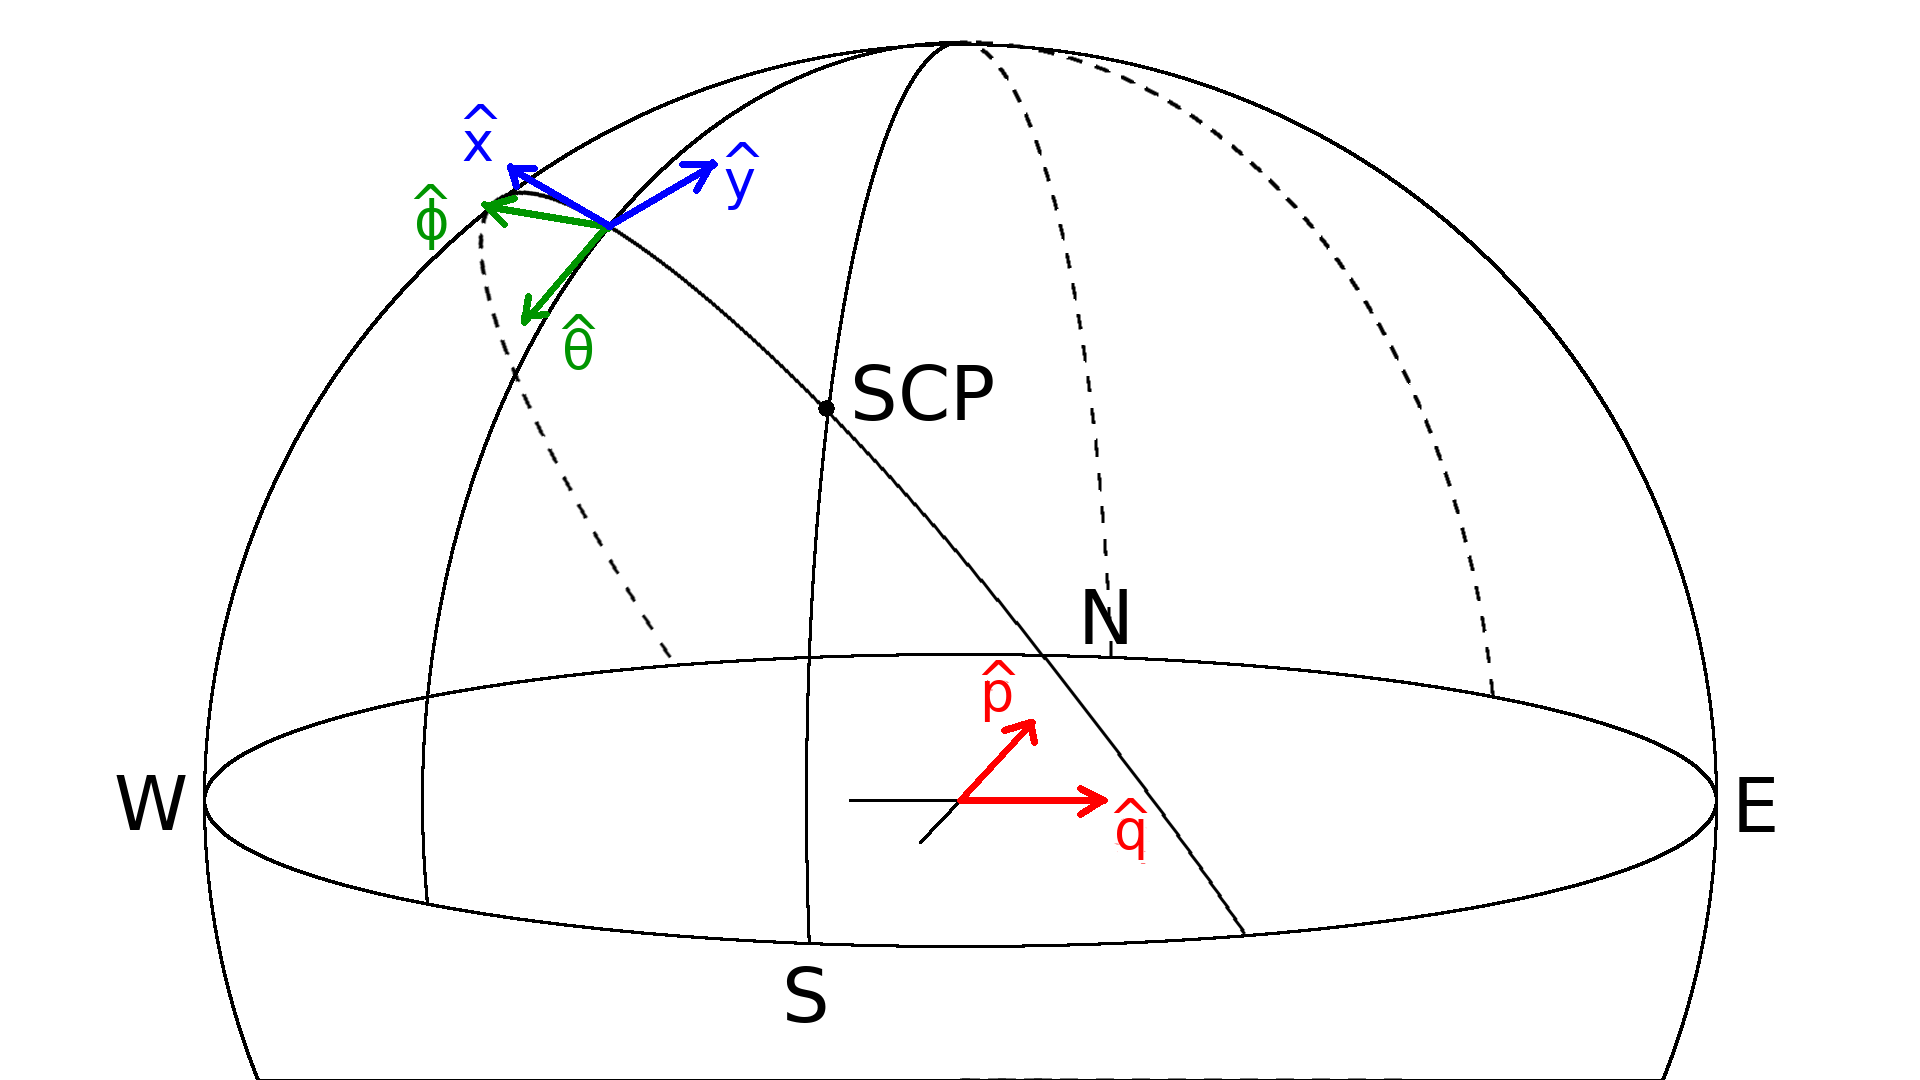
\includegraphics[width=\textwidth]{coords.png}
    \caption{Illustration of the three coordinate systems used in this documentation.}
    \label{fig:coords}
\end{figure}

\subsection{Instrumental coordinates}
\index{coordinates!instrumental}

This is a Cartesian coordinate system aligned with local (ground) compass directions.
Positive $p$ points towards local North, and positive $q$ towards local East.
The ``$P$ polarisation'' refers to the physical set of dipoles parallel to the N-S line; the ``$Q$ polarisation'', to the E-W line.

\subsection{Local sky coordinates}
\label{sec:coordslocalsky}
\index{coordinates!local sky}

This is a spherical coordinate system defined with respect to a local observer.
$\theta$ is the \textit{zenith angle}\index{zenith angle}, i.e. a \textit{colatitude}, with zenith itself therefore defined as $\theta = 0$ and the horizon as $\theta = \pi/2$.
$\phi$ is the \textit{azimuth}\index{azimuth}, and we define $\phi = 0$ in the North direction, with positive azimuth moving clockwise as viewed from above (i.e. N$\rightarrow$E$\rightarrow$S$\rightarrow$W$\rightarrow$N).
Moreover, the \textit{elevation}\index{elevation} is denoted by the symbol $\tilde{\theta}$, and is related to the zenith angle by
\begin{equation}
    \tilde{\theta} = \frac{\pi}{2} - \theta.
\end{equation}

\subsection{Celestial sky coordinates}
\index{coordinates!celestial sky}

This is a spherical coordinate system defined with respect to the celestial sphere.
$x$ is the \textit{declination}\index{declination} (Dec) and $y$ is the \textit{right ascension}\index{right ascension} (RA).

\subsection{Coordinate transformations}

%The three sets of coordinates described above span two-dimensional subspaces of the ambient three-dimensional space in which the celestial sphere and the telescope reside.
%Consequently, transformations between them generally require $3\times3$ matrices.
%If we define
%\begin{equation}
%    \begin{aligned}
%        \hat{s} \equiv \hat{p} \times \hat{q}, \\
%        \hat{r} \equiv \hat{\theta} \times \hat{\phi}, \\
%        \hat{z} \equiv \hat{x} \times \hat{y},
%    \end{aligned}
%\end{equation}
%then $(p,q,s)$, $(\theta,\phi,r)$, and $(x,y,z)$ are all three-dimensional, right-handed coordinate systems which are related by the following coordinate transformations:
%\begin{equation}
%    \begin{aligned}
%        \theta &= \arctan\left(-\frac{\sqrt{p^2 + q^2}}{s}\right) \\
%        \phi &= \arctan\left(\frac{q}{p}\right) \\
%        r &= -\sqrt{p^2 + q^2 + s^2}
%    \end{aligned}
%\end{equation}

All coordinate transformations can be effected by applying the appropriate Jacobian matrix for the desired transformation.
In this documentation, a boldface ${\bf P}$ will always be used\footnote{``${\bf J}$'' is reserved for (other) Jones matrices.} to denote such transformation matrices.
For general coordinates $(a,b)$ and $(c,d)$,
\begin{equation}
    \transmat{a}{b}{c}{d} =
    \begin{bmatrix}
        \pd{c}{a} & \pd{c}{b} \\[5 pt]
        \pd{d}{a} & \pd{d}{b}
    \end{bmatrix}
\end{equation}
Among these, the only transformation that is explicitly used in \vcsbeam{} is the transformation between local sky coordinates and celestial sky coordinates, which is a single rotation within the sky plane by the parallactic angle.

\subsubsection{Parallactic angle correction}

The parallactic angle correction is a transformation between local sky coordinates and celestial sky coordinates.
The parallactic angle itself, $\chi$, is defined as the position angle of local zenith with respect to the North Celestial Pole as subtended at a given source (see Fig. \ref{fig:skyangles}).
The transformation $(x,y)\rightarrow(\theta,\phi)$ is therefore a counterclockwise rotation\footnote{A counterclockwise rotation of a given vector is equivalent to a clockwise rotation of the coordinate axes.} by $\pi - \chi$.
This is the rotation
\begin{equation}
    \transmat{x}{y}{\theta}{\phi}
        = \begin{bmatrix}
            \cos\left(\pi - \chi\right) & -\sin\left(\pi - \chi\right) \\
            \sin\left(\pi - \chi\right) &  \cos\left(\pi - \chi\right)
        \end{bmatrix}
        = \begin{bmatrix}
            -\cos\chi & -\sin\chi \\
             \sin\chi & -\cos\chi
        \end{bmatrix}.
\end{equation}
\begin{figure}[!th]
    \centering
    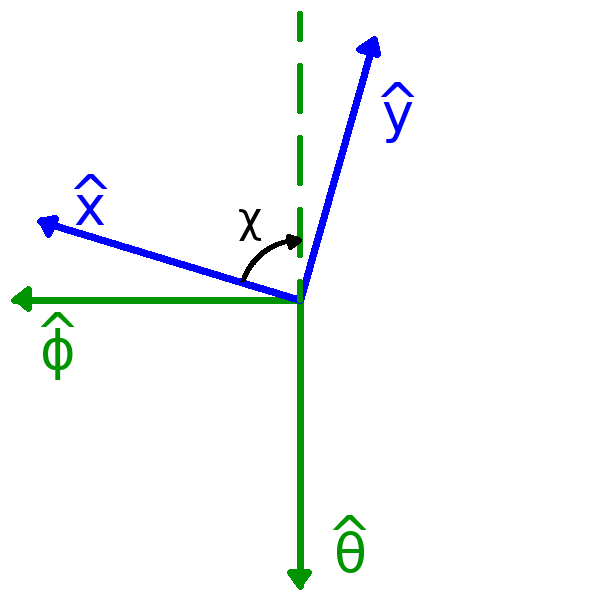
\includegraphics[width=0.4\textwidth]{skyangles.png}
    \caption{Definition of the parallactic angle, $\chi$, in the sky plane.}
    \label{fig:skyangles}
\end{figure}
The actual parallactic angle correction that is implemented is for historical reasons the matrix
\begin{equation}
    \pamat \equiv
    \transmat{y}{x}{\theta}{\phi}
        = \begin{bmatrix}
            -\sin\chi & -\cos\chi \\
            -\cos\chi &  \sin\chi
        \end{bmatrix}.
\end{equation}
In \vcsbeam{}, the parallactic angle is calculated (via the function \texttt{palPa} in the \href{https://github.com/Starlink/pal}{Starlink/pal} library) by the spherical triangle identity
\begin{equation}
    \tan \chi = \frac{\cos \lambda \sin H}{\sin\lambda \cos x - \cos \lambda \sin x \cos H},
\end{equation}
where $\lambda$ is the latitude of the observer\footnote{The latitude of the MWA is $\lambda_\text{MWA} = -0.4660608448386394\,$rad, defined in the \texttt{mwalib} library.}, $H$ is the hour angle of the source, and $x$ is the declination.

\chapter{Algorithms}

\section{PFB}

\subsection{Fine channelisation}

\section{Calibration}
\index{calibration}

Calibration is the process by which the temporal variations in the instrumental and/or ionospheric response to an incoming signal are characterised, in order to account for them when processing observational data.
A \textit{calibration solution} is a mathematical operation that can be applied either to measured visibilities or raw voltages to correct for these variations, and recover the visibilities (or raw voltages) that would have been measured under ideal conditions.

For the MWA, calibration solutions are modelled as a tile-dependent, linear transformation of two orthogonal polarisations.
Thus, the calibration solution for each tile is represented by a $2\times2$ Jones matrix, ${\bf D}$, which is left-multiplied (along with the primary beam correction, ${\bf B}$) to the incident electric field, ${\bf e}$, to predict the measured voltages, ${\bf v}$.
\begin{equation}
    {\bf v} = {\bf D}{\bf B}{\bf e}.
\end{equation}
Writing these matrices out in full, and using the canonical choice of bases\footnote{Different calibration software packages may use different coordinate bases.},
\begin{equation}
    \begin{bmatrix} v_p \\ v_q \end{bmatrix}
        = \begin{bmatrix}
            D_{pp} & D_{pq} \\
            D_{qp} & D_{qq}
        \end{bmatrix}
        \begin{bmatrix}
            B_{px} & B_{py} \\
            B_{qx} & B_{qy}
        \end{bmatrix}
        \begin{bmatrix} e_x \\ e_y \end{bmatrix},
\end{equation}
In practise, of course, the inverse opeations are used to reconstruct the electric field from the measured voltages:
\begin{equation}
    {\bf e} = {\bf B}^{-1}{\bf D}^{-1}{\bf v}.
\end{equation}
Generally, calibration is performed independently on individual frequency channels.

\subsection{Real Time Solution (RTS)}
\index{RTS}

The RTS is one of the pieces of software that can be used to generate calibration solutions for a VCS observation.
The solutions are given in two sets of files, called ``DI\_JonesMatrices\_nodeCCC.dat'' and ``BandpassCalibration\_nodeCCC.dat'' (CCC represents a coarse channel index).
These files contain the information needed to reconstruct the Jones matrices in the $(p,q)$ basis, which is required in order to take calibration solutions derived from one observation and apply (or ``transfer'') them to other observations.

The solutions are factored in the following way\footnote{It is as yet unclear if this gives a better result than ${\bf D} = ({\bf D}_d {\bf D}_b {\bf B}_\text{cal}^{-1})^*$.},
\begin{equation}
    {\bf D} = ({\bf D}_d {\bf D}_b)^* {\bf B}_\text{cal}^{-1},
    \label{eqn:rts_factorisation}
\end{equation}
where
\begin{itemize}
    \item ${\bf D}_d$ is the ``coarse channel tile gain''\index{gain} (one Jones matrix per tile, per coarse channel);
    \item ${\bf B}_\text{cal}$ is the ``alignment matrix''\index{alignment matrix}, or the primary beam model\index{primary beam} towards the calibrator source (one Jones matrix per coarse channel); and
    \item ${\bf D}_b$ is the ``bandpass gain'' (one Jones matrix per tile, per fine channel).
\end{itemize}

\subsubsection{Coordinate bases}

The coordinate bases for the various RTS matrices described in this section are not well-documented elsewhere, and are mainly assumed to be correct based on empirical tests performed on actual observations of pulsars.
Having said that, one of the early plotting scripts designed to visualise the RTS calibration solutions matrices is suggestive that
\begin{enumerate}
    \item ${\bf D}_d$ is in the basis $(x,y)\rightarrow(p,q)$,
    \item ${\bf D}_b$ is in the basis $(x,y)\rightarrow(x,y)$,
    \item ${\bf B}_\text{cal}$ is in the basis $(p,q)\rightarrow(x,y)$.
\end{enumerate}
This would put the resulting ${\bf D}$ matrix in the basis:
\begin{equation}
    {\bf D} = \begin{bmatrix}
        D_{pp} & D_{pq} \\
        D_{qp} & D_{qq}
    \end{bmatrix}.
\end{equation}
However, the current implementation in the beamformer does the following sequence of operations.
After obtaining ${\bf D}$ from the RTS output files according to Eq.~\eqref{eqn:rts_factorisation}, it is multiplied to the primary beam to produce the final Jones matrix:
\begin{equation}
    {\bf J} = {\bf D}{\bf B}\pamat.
\end{equation}
The primary beam is obtained using \href{https://github.com/MWATelescope/mwa_hyperbeam}{Hyperbeam}, which is based on the FEE beam model\index{primary beam!full embedded element (FEE)} \citep{Sokolowski2017}.
According to the documentation, this gives the ${\bf B}$ matrix in the $(\theta,\phi)\rightarrow(q,p)$ basis.
Since, by inspection of actual calibration solutions, the ${\bf D}$ matrices have the elements with the largest moduli along the main diagonal, we infer that the ${\bf D}$ matrices maintain the same basis, and that, despite what the plotting scripts suggest, the ${\bf D}$ is in fact
\begin{equation}
    {\bf D} = \begin{bmatrix}
        D_{qq} & D_{qp} \\
        D_{pq} & D_{pp}
    \end{bmatrix}.
\end{equation}
This agrees with the code in the \texttt{invj\_the\_data()} GPU kernel, which applies


As argued above, the $\pamat$ matrix embodies the transformation $(y,x)\rightarrow(\theta,\phi)$.
Taken together, 

\subsection{Hyperdrive}

\section{Beamforming}

\section{Applications}

\section{Utilities}

\chapter{Implementation}

\section{Code glossary}

\subsection{\texttt{az}}
\begin{description}
    \item[Name:] \hyperlink{sec:coordslocalsky}{Geographic azimuth}\index{azimuth!geographic}
    \item[Units:] radians
    \item[Functions:] \hyperlink{cn:calc_beam_geom}{\texttt{calc\_beam\_geom}}
\end{description}

\subsection{\texttt{el}}
\begin{description}
    \item[Name:] \hyperlink{sec:coordslocalsky}{Elevation}\index{elevation}
    \item[Units:] radians
    \item[Functions:] \hyperlink{cn:calc_beam_geom}{\texttt{calc\_beam\_geom}}
\end{description}

\subsection{\texttt{za}}
\begin{description}
    \item[Name:] \hyperlink{sec:coordslocalsky}{Zenith angle}\index{zenith angle}
    \item[Units:] radians
    \item[Functions:] \hyperlink{cn:calc_beam_geom}{\texttt{calc\_beam\_geom}}
\end{description}

\section{Function reference}

\subsection{\texttt{calc\_beam\_geom}}
\label{fcn:calc_beam_geom}

\appendix

\chapter{Description of RTS DI\_JonesMatrix file format}

\begin{lstlisting}
Franz Kirsten <franz.kirsten@curtin.edu.au>	17 June 2016 at 17:42
To: Sammy McSweeney <sammy.mcsweeney@gmail.com>, Steven Tremblay <Steven.Tremblay@curtin.edu.au>, Dr Stephen ORD <steve.ord@gmail.com>
Hi Sam,

Mitch finally got back to me on my questions about the individual entries in the DI_Jones matrices as output by the RTS. If you have a chance, could you go through those and try to get Andre's solutions to work once more? Are Mitch's answers enough or do you need more details?

It would be great if you could tell people next week that the beamformer also works with those tools now -- no pressure ;)

Cheers,
Franz




Hi Franz,

Sorry for the delay. Once you have this working I will let you know how to include the bandpass data.

Mitch

In an effort to automate calibrating the MWA for the tied-array beam, we
are currently trying to compare the the DI-Jones matrices from the RTS
with those produced by Andre Offringa's 'calibrate'. We know exactly
what is in Andre's solutions but are unsure about the
structur/formatting of the RTS solutions. Could you give a detailed
breakdown, please? In particular we were wondering about the following:

1) What is the number in the very first line?

This is the flux density of the calibrator that was used. You can ignore it.

The second line contains the model primary beam Jones matrix (in the direction of the calibrator).

2) Which column contains real/imaginary xx/yy/xy/yx?

XX_re XX_im XY_re XY_im YX_re YX_im YY_re YY_im

3) Are the numbers normalised in some way?

By the model primary beam Jones matrix (from the second line). If that is called B, and the direction-independent gain for tile i is G_i, then the numbers printed are G_i.B (call this J_i). So to get the direction-independent gain to compare with Andre's: G_i = J_i.inv(B).

4) Is there some conjugation going on?

No.
\end{lstlisting}

\chapter{Description of RTS BandpassCalibration file format}

\begin{lstlisting}
Sammy McSweeney <sammy.mcsweeney@gmail.com>	21 March 2017 at 12:09
To: Daniel.Mitchell@csiro.au, Franz Kirsten <franz.kirsten@curtin.edu.au>, Steven Tremblay <Steven.Tremblay@curtin.edu.au>
Hi Mitch,

Thanks for your explanation (via Franz, last year) of how the DIJones RTS output files are organised. If I could trouble you now for a similar explanation for how the Bandpass files are organised...
As far as I can make out, the format is something like:

freq00 freq01 freq02 ... (minus any flagged channels)
tilenum amp,phase, amp,phase, amp,phase, ...
tilenum amp,phase, amp,phase, amp,phase, ...
etc ...

I see that there are 8 rows per tile, but I'm not how those 8 break down (into polarisation combinations, for example). Incidentally, what do the "P" and "Q" mean in "PX", etc? (I see it cropping up in some of Steve Ord's plotting scripts.)

And, calling in your promised favour, anything you can tell me about "how to include the bandpass data" would be much appreciated.

Cheers,
~/Sam
\end{lstlisting}

\begin{lstlisting}
Daniel.Mitchell@csiro.au <Daniel.Mitchell@csiro.au>	23 March 2017 at 06:55
To: sammy.mcsweeney@gmail.com
Cc: franz.kirsten@curtin.edu.au, Steven.Tremblay@curtin.edu.au
Hi Sammy,

There are 8 lines for each antenna: Jm[0],Jf[0],Jm[1],Jf[1],Jm[2],Jf[2],Jm[3],Jf[3], where Jm contains the measured Jones matrices (measured separately for each frequency channel), and Jf contains low-order fits to these data, which are used in the RTS as the bandpass solutions (polynomials are fitted separately to the real and imaginary components of each Jones matrix element).

P and Q are the labels that we use for the two instrument polarisations (North-South and East-West respectively). X and Y are the standard sky polarisation coordinates, with X aligned with declination and Y aligned with RA.

The overall Jones matrix for a given channel of a given antenna will be the full-band matrix from the DIJones file multiplied by the bandpass matrix on the righthand side.

Cheers,
Mitch
\end{lstlisting}

\chapter{Comparison of notation in other documents}

\section{Coordinate systems}

\begin{table}[!hb]
    \centering
    \caption{Comparison of coordinate notations}
    \label{tbl:notations}
    \begin{tabular}{l|cc|cc|cc}
        This document & $p$ & $q$ & $\theta$ & $\phi$ & $x$ & $y$ \\
        \hline
        MWA metafits files       & X & Y & - & - & - & - \\
        \citet{Sokolowski2017} & $y$ & $x$ & $\theta$ & $\phi$ & - & - \\
    \end{tabular}
\end{table}

The apparent reversal of the metafits files polarisations compared to the \citet{Sokolowski2017} notation is put here only very reluctantly.
This is also at odds with conversations with various MWA Operations team members, who insist that `X' aligns E-W and `Y' aligns N-S.
Nevertheless, \vcsbeam{} appears to only produce sensible results when I treat the voltages listed under `X' in the metafits file as if they were those measured with the N-S dipole, and `Y' with the E-W dipole.
It remains to be seen whether this holds true for MWAX data, since it may turn out, for example, that the role of the polarisations is inadvertently swapped during the recombine process.

\section{Jones matrices}

\begin{table}[!hb]
    \centering
    \caption{Comparison of matrix names}
    \label{tbl:notations}
    \begin{tabular}{l|ccc}
        This document & ${\bf J}$ & ${\bf D}$ & ${\bf B}$ \\
        \hline
        \citet{Sokolowski2017} & ${\bf J}$ & ${\bf G}$ & ${\bf E}$ \\
    \end{tabular}
\end{table}

\printindex

\bibliography{vcsbeam_documentation}

\end{document}
